\documentclass[11pt, oneside]{article}
\usepackage{geometry}
\geometry{letterpaper}
\usepackage{graphicx}
\usepackage{amssymb}
\usepackage{amsmath}
\usepackage{tikz}
\usepackage{tikz-qtree}
\usepackage{url}

\title{SICP Exercise 3.10}
\author{Yuchong Pan}

\begin{document}
\maketitle

The environments created by evaluating (define W1 (make-withdraw 100)) are given as follows:

\begin{center}
    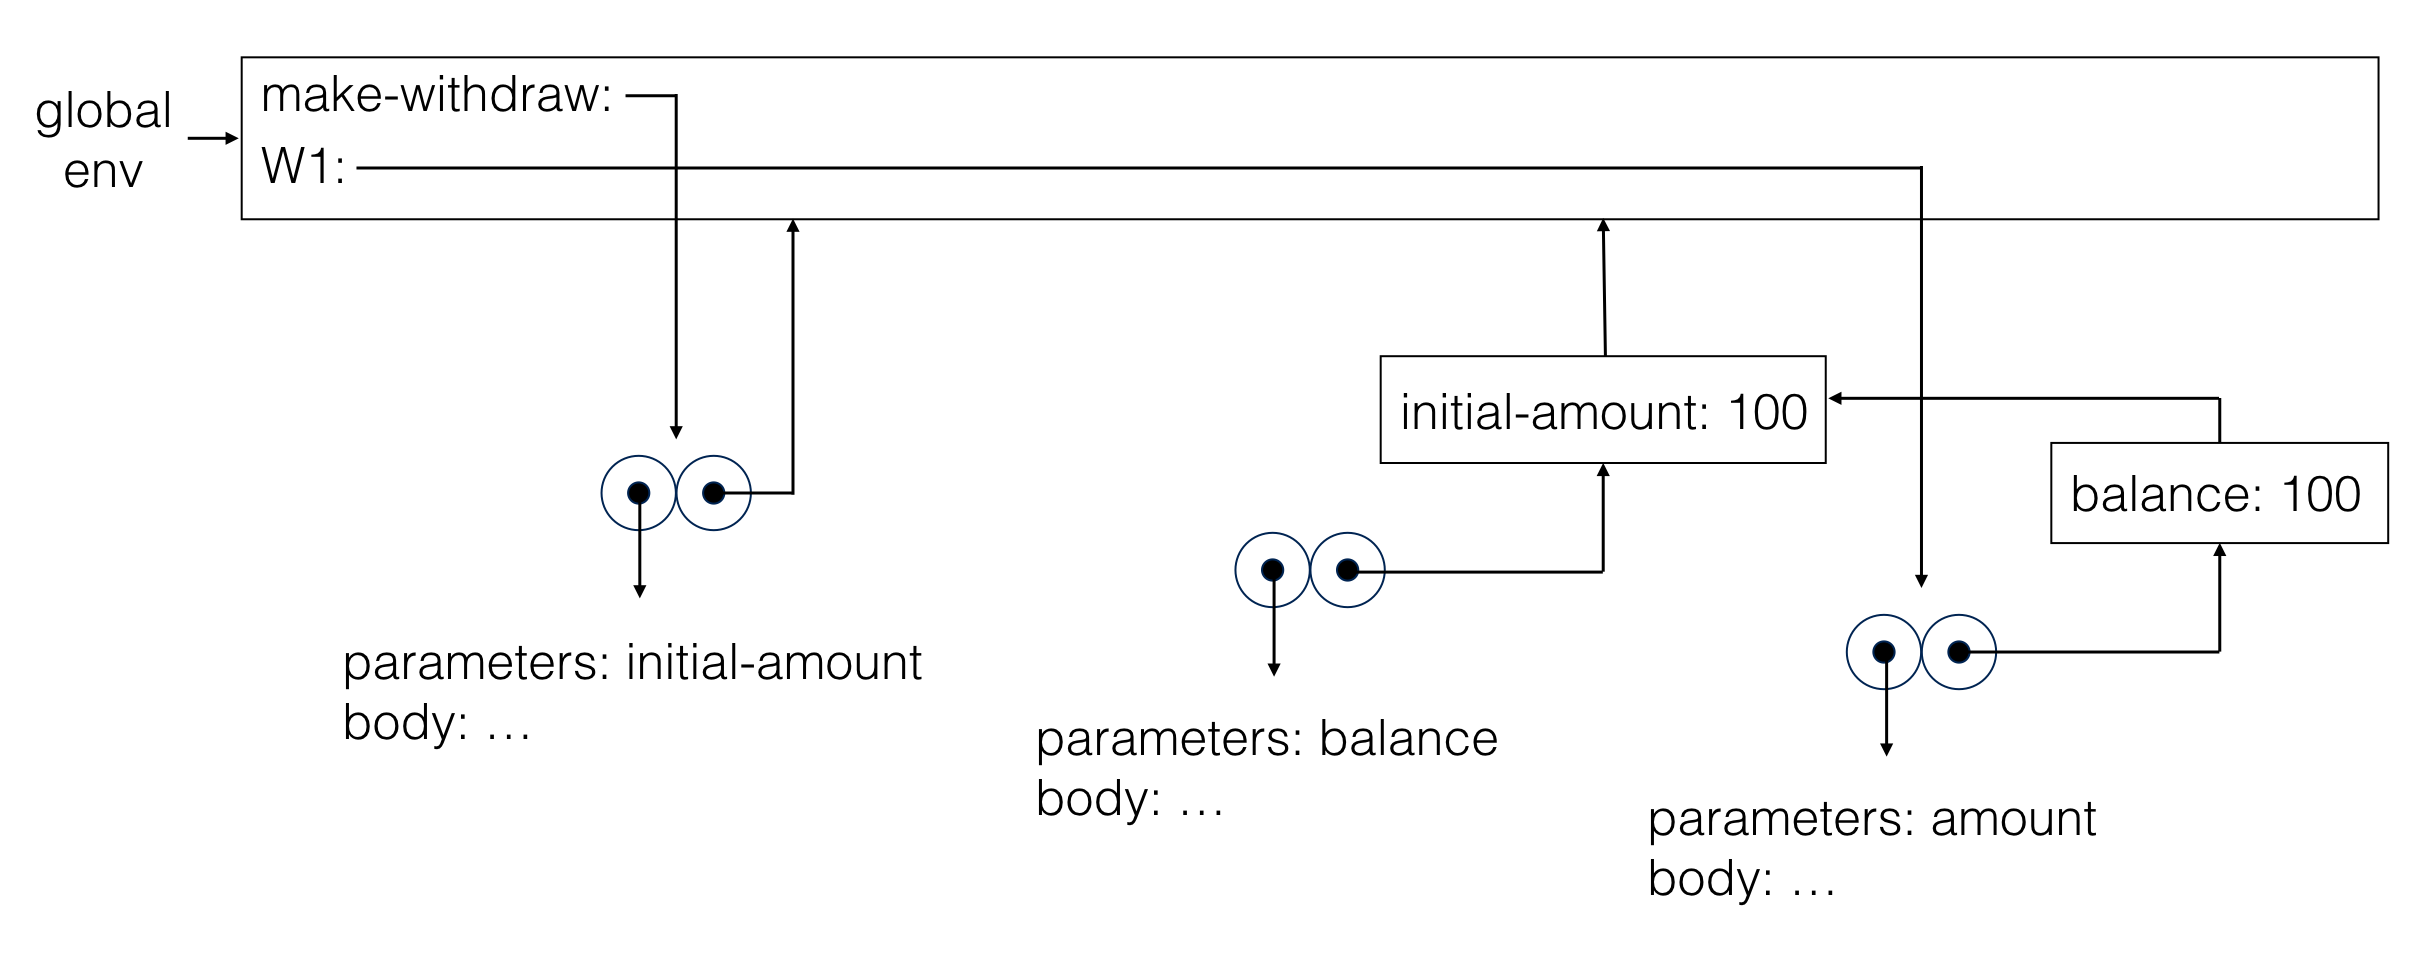
\includegraphics[width=15cm]{ex-3.10-1.png}
\end{center}

The environments created by applying the procedure object W1 to 50 are given as follows:

\begin{center}
    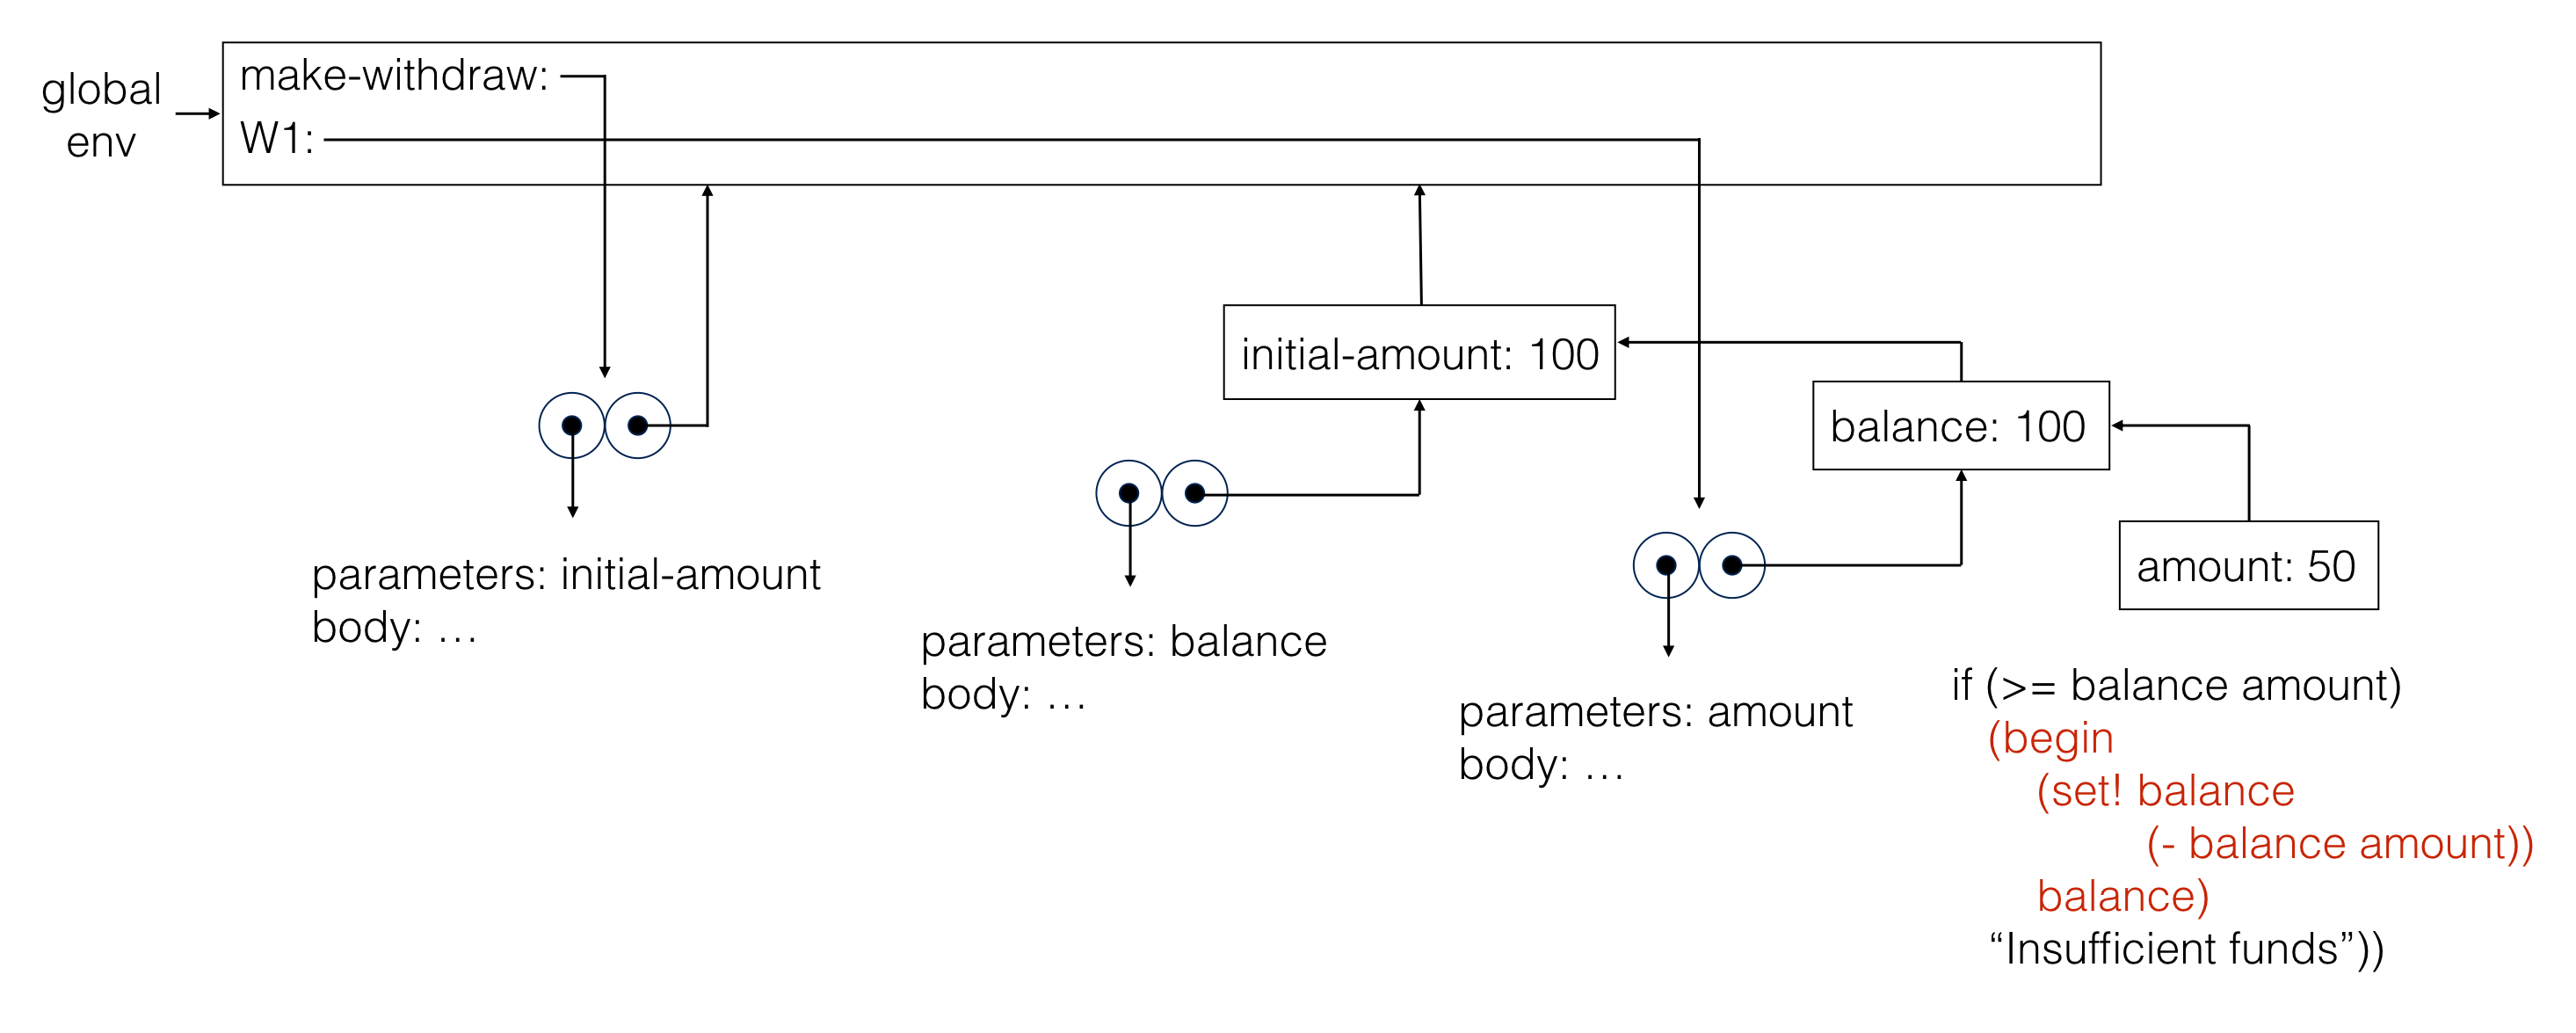
\includegraphics[width=15cm]{ex-3.10-2.png}
\end{center}

After the call to W1, the environments become

\begin{center}
    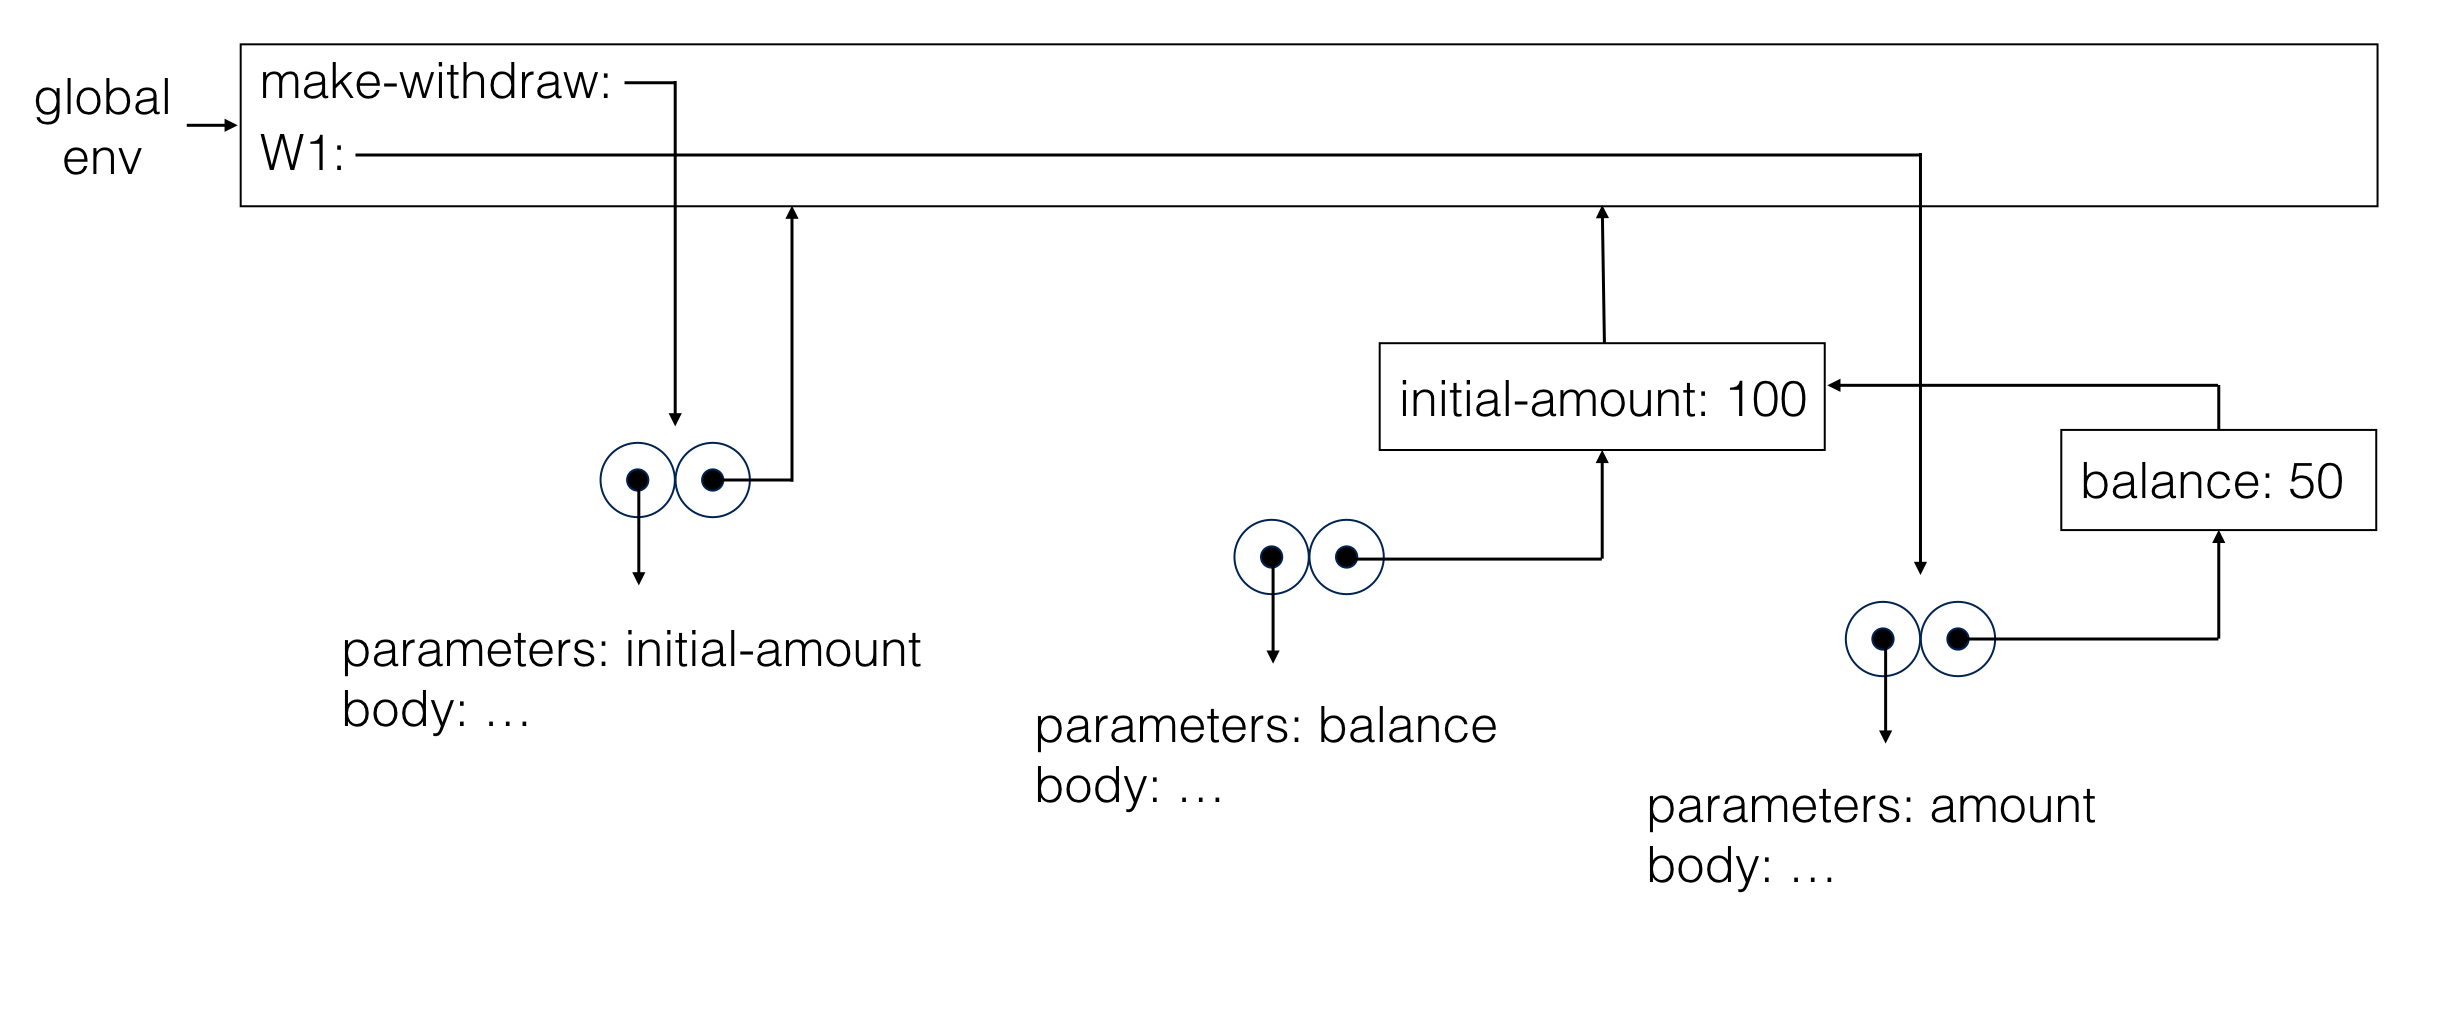
\includegraphics[width=15cm]{ex-3.10-3.png}
\end{center}

Using (define W2 (make-withdraw 100)) to create a second object gives

\begin{center}
    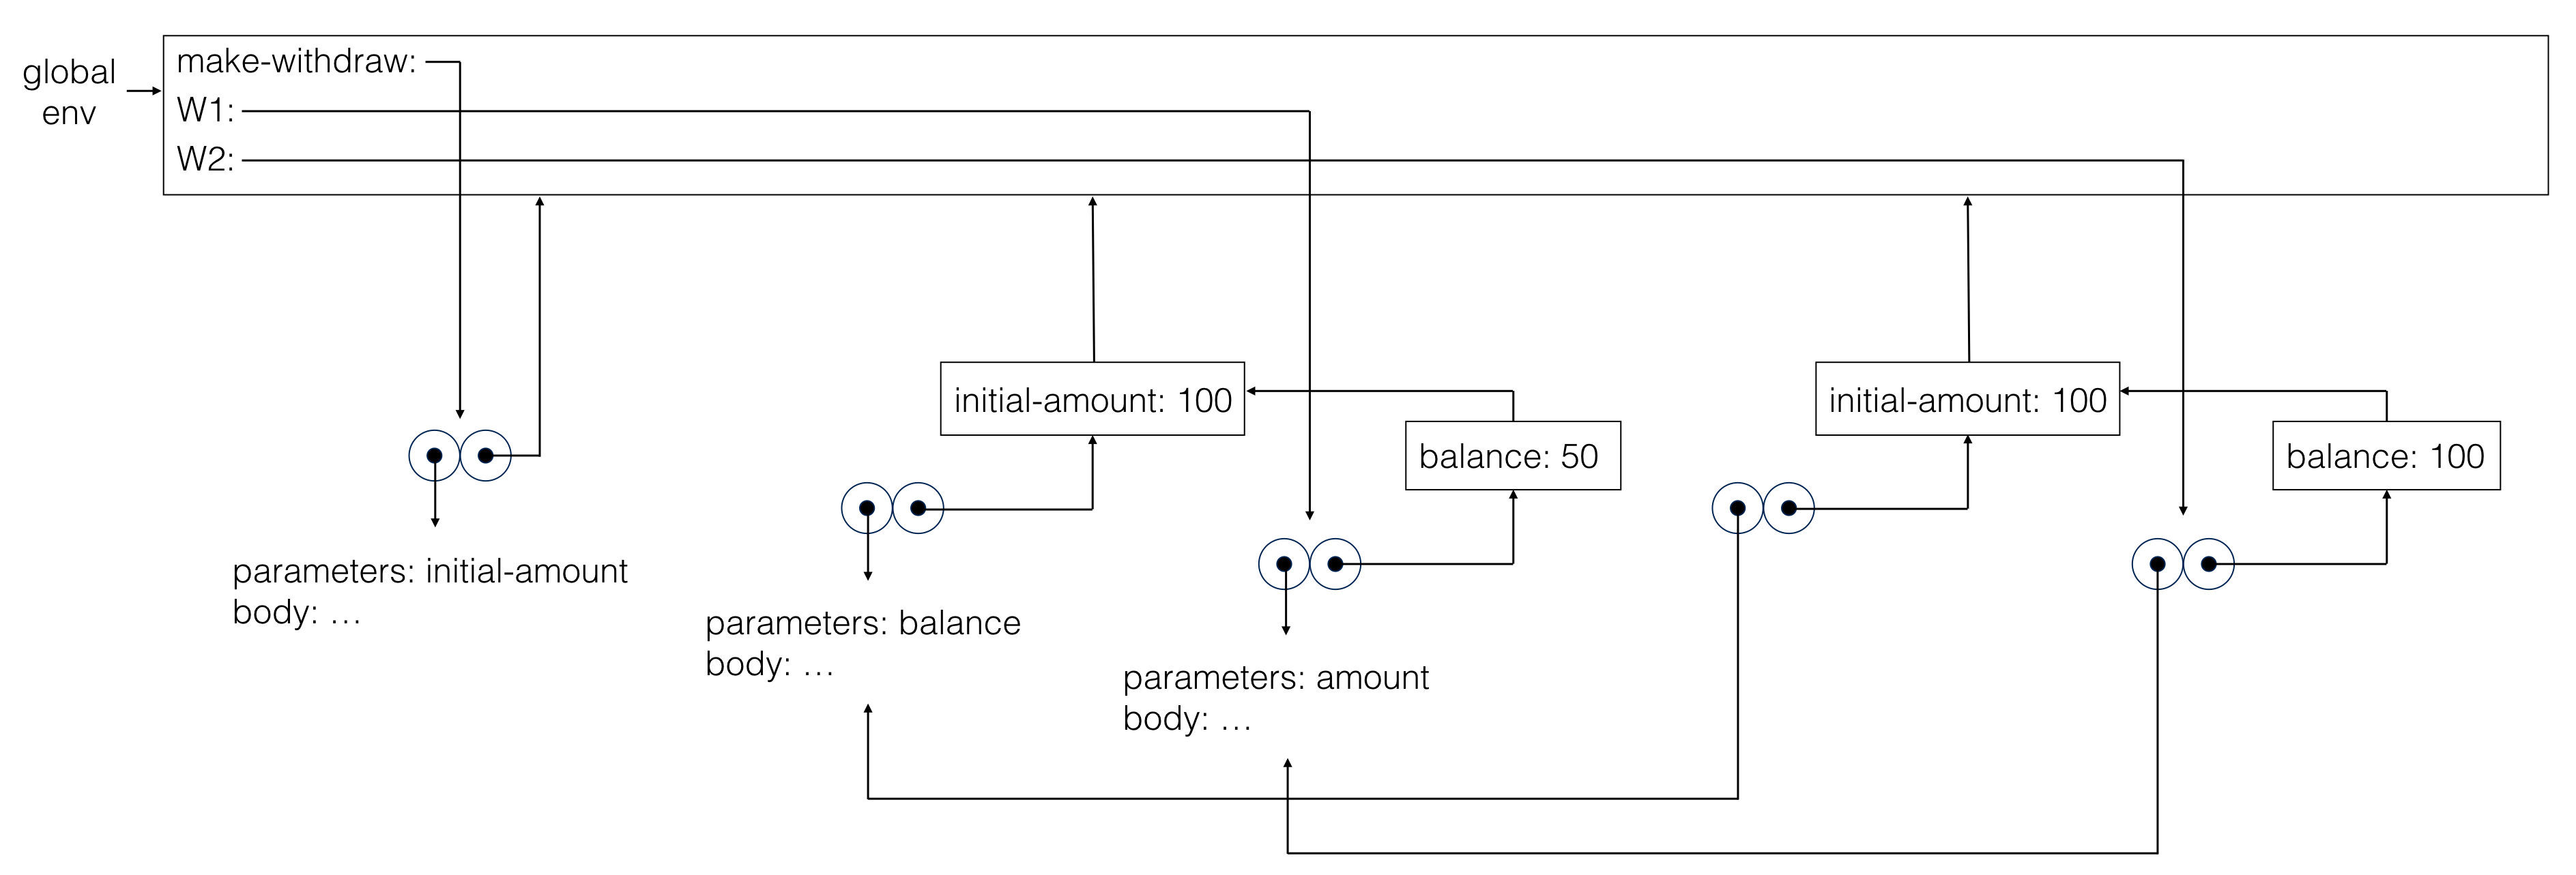
\includegraphics[width=15cm]{ex-3.10-4.png}
\end{center}

The two versions of \url{make-withdraw} create objects with the same behavior, since the environments created by the two versions of \url{make-withdraw} each contain a frame with its own local binding for \url{balance}, and since he state variables \url{make-withdraw} which calls to \url{W1} and to \url{W2} reference are stored in different environments.

By contrast, the environment structures created by the alternate version have an extra "anonymous" procedure object and an extra frame with the binding for \url{initial-amount} for each object created by \url{make-withdraw}. Hence, more space is required for the latter version.

\end{document}
